\documentclass[11pt]{article}

\usepackage[margin=1in]{geometry}
\usepackage[T1]{fontenc}
\usepackage{lmodern}
\usepackage{microtype}
\usepackage{parskip}
\usepackage{amsmath, amssymb, mathtools}
\usepackage{siunitx}
\usepackage{graphicx}
\usepackage{float}
\usepackage[justification=centering]{caption}
\usepackage{booktabs}
\usepackage{xcolor}
\usepackage{hyperref}
\usepackage{fancyhdr}
\usepackage{lastpage}

\newcommand{\nlinksP}{7}
\newcommand{\LlinkP}{3.505}
\newcommand{\MjP}{518.4}
\newcommand{\kkP}{0.437}
\newcommand{\MkzeroP}{0.229}
\newcommand{\QfricP}{2.67}
\newcommand{\ImaxaP}{7.39e+05}
\newcommand{\ImaxbP}{6.91e+05}
\newcommand{\TaOneP}{6594}
\newcommand{\TbOneP}{15172}
\newcommand{\TtotOneP}{21766}
\newcommand{\TaFiveP}{2949}
\newcommand{\TbFiveP}{6785}
\newcommand{\TtotFiveP}{9734}
\newcommand{\TaTenP}{2085}
\newcommand{\TbTenP}{4798}
\newcommand{\TtotTenP}{6883}
\newcommand{\TnP}{3.09e+03}
\newcommand{\tfreeP}{786}
\newcommand{\wfreeP}{0.0124}
\newcommand{\KEfreeP}{3.63}
\newcommand{\EspringP}{3.77}
\newcommand{\WfricP}{3.72}
\newcommand{\marginAP}{1.22}
\newcommand{\marginBP}{5.84}
\newcommand{\ratioAP}{3.4e-02}
\newcommand{\ratioBP}{1.5e-03}
\newcommand{\TnratioP}{1.17}
\newcommand{\recTaP}{7200}
\newcommand{\recTbP}{16200}
\newcommand{\recTtotP}{23400}
\newcommand{\recRaP}{0.84}
\newcommand{\recRbP}{0.88}
\newcommand{\recRaHumanP}{2}
\newcommand{\recRbHumanP}{4.5}
\newcommand{\recTotHumanP}{6.5}
\newcommand{\curRaP}{3.35}
\newcommand{\curRbP}{0.147}
\newcommand{\nlinksB}{2}
\newcommand{\LlinkB}{0.254}
\newcommand{\MjB}{1.062}
\newcommand{\kkB}{0.0273}
\newcommand{\MkzeroB}{0.0143}
\newcommand{\QfricB}{0.0476}
\newcommand{\ImaxaB}{0.254}
\newcommand{\ImaxbB}{0.245}
\newcommand{\TaOneB}{28.7}
\newcommand{\TbOneB}{63.4}
\newcommand{\TtotOneB}{92.0}
\newcommand{\TaFiveB}{12.8}
\newcommand{\TbFiveB}{28.3}
\newcommand{\TtotFiveB}{41.2}
\newcommand{\TaTenB}{9.1}
\newcommand{\TbTenB}{20.0}
\newcommand{\TtotTenB}{29.1}
\newcommand{\TnB}{13.5}
\newcommand{\tfreeB}{3.77}
\newcommand{\wfreeB}{1.04}
\newcommand{\KEfreeB}{0.0648}
\newcommand{\EspringB}{0.0673}
\newcommand{\WfricB}{0.0665}
\newcommand{\marginAB}{281}
\newcommand{\marginBB}{1.4e+03}
\newcommand{\ratioAB}{6.3e-07}
\newcommand{\ratioBB}{2.6e-08}
\newcommand{\TnratioB}{266}
\newcommand{\recTaB}{30.0}
\newcommand{\recTbB}{65.0}
\newcommand{\recTtotB}{95.0}
\newcommand{\recRaB}{0.91}
\newcommand{\recRbB}{0.95}
\newcommand{\recRaHumanB}{0.0083}
\newcommand{\recRbHumanB}{0.018}
\newcommand{\recTotHumanB}{0.0264}
\newcommand{\curRaB}{0.00}
\newcommand{\curRbB}{0.000}


\newcommand{\Name}{Arael Anaya}
\newcommand{\dth}{\dot{\theta}}
\newcommand{\ddth}{\ddot{\theta}}
\newcommand{\st}{\sin\theta}
\newcommand{\ct}{\cos\theta}
\newcommand{\Ieff}{I_{\text{eff}}}

\pagestyle{fancy}
\fancyhf{}
\lhead{Deployment Time Decision | Senior Design}
\rhead{\Name\ | \today}
\cfoot{Page \thepage\ of~\pageref{LastPage}}
\hypersetup{colorlinks, linkcolor={red!50!black}, urlcolor={blue!80!black}}

\title{Deployment Time Selection\\
\large Minimum deployment time that permits the quasi-static model}
\author{\Name}
\date{\today}

\begin{document}
\maketitle

\section{Decision}

The quasi-static equation of motion (Derivation, Sec.~``Quasi-Static Assumption'') drops the
$\Ieff\ddth$ and $M_j S_1 L^2\st\ct\,\dth^2$ terms. That is only valid if each deployment phase is
\emph{slow enough}. Requiring the peak inertial torque to stay below a fraction $\varepsilon$ of the
hinge friction torque $N_s\tau_f$ gives a minimum duration for each phase. I take
$\varepsilon=1\%$ as the design target and report $5\%$ and $10\%$ for reference.

\begin{table}[H]
\centering
\caption{Minimum phase duration $T_{\min}$ so that inertial torque $\le\varepsilon\,N_s\tau_f$.}
\begin{tabular}{@{}l l r r r@{}}
\toprule
 & $\varepsilon$ & Phase 1 (s) & Phase 2 (s) & Total (s) \\
\midrule
Production (orbit) & 10\% & \TaTenP & \TbTenP & \TtotTenP \\
 & 5\%  & \TaFiveP & \TbFiveP & \TtotFiveP \\
 & 1\%  & \TaOneP & \TbOneP & \TtotOneP \\
\midrule
Bench test & 10\% & \TaTenB & \TbTenB & \TtotTenB \\
 & 5\%  & \TaFiveB & \TbFiveB & \TtotFiveB \\
 & 1\%  & \TaOneB & \TbOneB & \TtotOneB \\
\bottomrule
\end{tabular}
\end{table}

\textbf{Recommended deployment time ($\varepsilon\approx1\%$ in both phases):}
\begin{itemize}
  \item \textbf{Production:} Phase~1 $=\recRaHumanP$~h, Phase~2 $=\recRbHumanP$~h, total
        $\approx\recTotHumanP$~h. Inertial-to-friction torque is then \recRaP\% (Phase~1) and
        \recRbP\% (Phase~2). This fits inside the 12~h budget in \texttt{params.py} with about 1.8$\times$ schedule margin.
  \item \textbf{Bench test:} Phase~1 $=\recTaB$~s, Phase~2 $=\recTbB$~s (about 1.6~min total), giving \recRaB\% and \recRbB\%.
  \item \textbf{The 1~h / 11~h split currently in \texttt{params.py} should change.} Phase~1 is
        binding: at 1~h its inertial torque is \curRaP\% of friction, versus \curRbP\% for Phase~2 at 11~h. Move time from Phase~2 to Phase~1 (for example 2~h / 4.5~h, or 3~h / 9~h if the full 12~h is kept).
  \item \textbf{Deployment must be rate-limited.} The springs alone deploy the array in
        \tfreeP~s (production) or \tfreeB~s (bench) if left free-running (Sec.~\ref{sec:free}),
        far below $T_{\min}$. The quasi-static model only holds if something (damper, metered
        release, controlled inflation rate) holds deployment to the durations above.
\end{itemize}

\section{Which terms are neglected}

The full equation of motion (Derivation) is
\begin{equation}
\underbrace{\big[M_j S_1 L^2\sin^2\theta + n I_j + \tfrac12 n M_j L^2\big]}_{\Ieff(\theta)}\ddth
+ M_j S_1 L^2\st\ct\,\dth^2 + N_s k\theta + 2N_k M_k = N_s\tau_f .
\end{equation}
Quasi-static deployment drops the first two terms (angular acceleration and rate-squared). No other
dynamic effect is in the model; the ones \emph{not} covered here are listed in Sec.~\ref{sec:caveats}.

\section{Method}

Each phase sweeps an angle $\Delta\theta$ in time $T$: Phase~1 from $\theta_0=90^\circ$ to
$\theta_1=75^\circ$ ($\Delta\theta=15^\circ$), Phase~2 from $\theta_1$ to $\theta_{\min}=10^\circ$
($65^\circ$). To bound the peaks I use a minimum-jerk profile
$\theta(t)=\theta_a+\Delta\theta(10s^3-15s^4+6s^5)$, $s=t/T$, which starts and ends at rest. Its
peak rate and acceleration are
\begin{equation}
|\dth|_{pk}=1.875\,\frac{\Delta\theta}{T},\qquad |\ddth|_{pk}=5.774\,\frac{\Delta\theta}{T^2}.
\end{equation}
The peak inertial torque, with the two terms added (conservative, since they do not peak together), is
\begin{equation}
\tau_{in}(T)\le \Ieff^{\max}\,5.774\,\frac{\Delta\theta}{T^2}
 + M_j S_1 L^2\,(\st\ct)^{\max}\Big(1.875\frac{\Delta\theta}{T}\Big)^2
 \equiv \frac{c}{T^2},
\end{equation}
where $\Ieff^{\max}$ and $(\st\ct)^{\max}$ are taken over the phase's angle range.
Both terms scale as $1/T^2$, so the ratio to friction and the minimum time are
\begin{equation}
\frac{\tau_{in}}{N_s\tau_f}=\frac{c/(N_s\tau_f)}{T^2}\le\varepsilon
\;\;\Longrightarrow\;\;
\boxed{T_{\min}=\sqrt{\frac{c}{\varepsilon\,N_s\tau_f}}}\ .
\end{equation}
Friction is the reference because it is the load the quasi-static balance
$N_s k\theta+2N_kM_k=N_s\tau_f$ must overcome, and the springs and kink are sized to exceed it
($k=1.5\,\tau_f/\theta_1$, $M_{k0}=1.5\,N_s(\tau_f-k\theta_{\min})/2N_k$, Derivation Secs.~PHASE~1--2).
$\tau_f$ is the design value $1.5\times5\,\mathrm{N}\times r_o$ from \texttt{params.py}.

\subsection*{Inputs (from \texttt{params.py} / \texttt{testingParams.py})}

\begin{table}[H]
\centering
\begin{tabular}{@{}l r r@{}}
\toprule
 & Production & Bench \\
\midrule
Links $n$ & \nlinksP & \nlinksB \\
Link length $L$ (m) & \LlinkP & \LlinkB \\
Mass per link $M_j$ (kg) & \MjP & \MjB \\
$\Ieff^{\max}$, Phase 1 / 2 (kg\,m$^2$) & \ImaxaP\ / \ImaxbP & \ImaxaB\ / \ImaxbB \\
Friction torque $N_s\tau_f$ (N\,m) & \QfricP & \QfricB \\
Hinge spring rate $k$ (N\,m/rad) & \kkP & \kkB \\
Kink moment $M_{k0}$ (N\,m) & \MkzeroP & \MkzeroB \\
\bottomrule
\end{tabular}
\end{table}

\section{Results}

\begin{figure}[H]
\centering
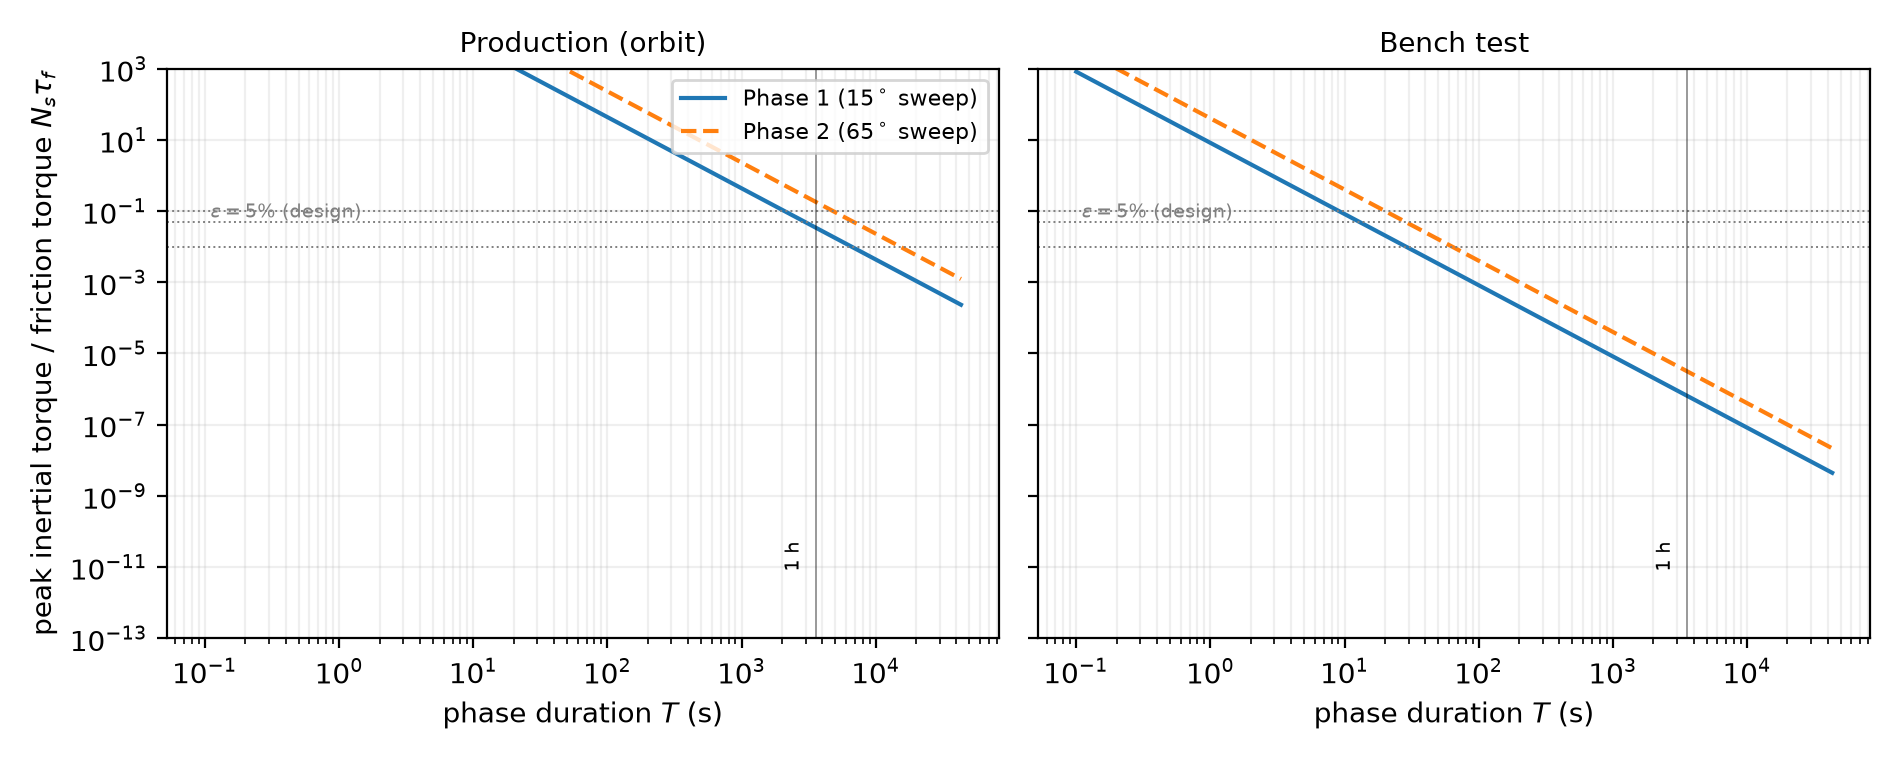
\includegraphics[width=\linewidth]{fig_ratio_vs_time.png}
\caption{Peak inertial torque as a fraction of friction torque versus phase duration. Dotted
lines mark 1\%, 5\% and 10\%. Phase~1 (solid) is always the more demanding phase.}
\end{figure}

\begin{itemize}
  \item Phase~1 sets the schedule even though its sweep is smaller, because its acceleration term
        scales with $\Delta\theta/T^2$ and the current split gives it only 1/12 of the time.
  \item Production at the current 1~h / 11~h split: \curRaP\% (Phase~1) and \curRbP\% (Phase~2).
        Phase~1 clears the 5\% line by only $\marginAP\times$ in time.
  \item Bench at 1~h / 11~h would be $\ratioAB$ / $\ratioBB$, i.e.\ trivially quasi-static. The
        bench test does not need hours. \TtotOneB~s total is enough.
\end{itemize}

\section{Cross-checks}

\subsection{Natural period}

The spring--inertia mode has period $T_n=2\pi\sqrt{\Ieff^{\max}/(N_sk)}$ = \TnP~s (production) and
\TnB~s (bench). A load applied over a time comparable to $T_n$ or longer does not excite that mode,
so $T\gtrsim T_n$ is the standard quasi-static criterion. The 5\% minimum times above are
$0.95$--$2.2\,T_n$ for both sets, so the two independent criteria agree. Production phases
of \recRaHumanP~h and \recRbHumanP~h are $2.3\,T_n$ and $5.2\,T_n$.

\subsection{Free-running deployment}\label{sec:free}

Integrating the full equation of motion from rest at stow with springs, friction and the kink
moment, and no rate limiter, gives

\begin{table}[H]
\centering
\begin{tabular}{@{}l r r@{}}
\toprule
 & Production & Bench \\
\midrule
Free-running deployment time (s) & \tfreeP & \tfreeB \\
Speed at $\theta_{\min}$ (rad/s) & \wfreeP & \wfreeB \\
Kinetic energy at end of travel (J) & \KEfreeP & \KEfreeB \\
Stored spring energy at stow (J) & \EspringP & \EspringB \\
\bottomrule
\end{tabular}
\end{table}

Both are well below $T_{\min}$, so with only 1.5$\times$ margin on the friction floor the array
deploys under inertia, not quasi-statically. The end-of-travel kinetic energy is comparable to the
entire stored spring energy, which is what the deployed latch would have to absorb. A rate limiter
that stretches deployment to at least the durations recommended above removes both problems.

\subsection{Sensitivity to friction}

Since $T_{\min}\propto(N_s\tau_f)^{-1/2}$, halving the friction estimate raises every time by
$1.41\times$ and doubling it lowers them by $0.71\times$. The bench friction budget
(\texttt{Friction Table/friction\_budget.py}, nominal case) gives a resistive torque of about
0.43--0.50~N\,m against the 0.048~N\,m used here, so the bench $T_{\min}$ values above are
conservative by roughly $3\times$ if that budget is right. The production friction budget was not run
here (the script follows \texttt{USE\_TESTING\_PARAMS}), so the production values rest on the
5~N placeholder.

\section{Issues found in the existing files}\label{sec:issues}

\begin{itemize}
  \item \textbf{Derivation, Quasi-Static section.} The text says inertial terms are
        ``$10^3$--$10^4\times$ smaller than every other torque.'' The table in that section shows
        $5.6\times10^{-3}$ for Phase~1 (about $180\times$ smaller). With the minimum-jerk peaks used here it is
        \ratioAP\ (about $30\times$). The claim holds for Phase~2 but not Phase~1.
  \item \textbf{\texttt{quasi\_static\_check.py}} estimates rates as $\Delta\theta/T$ and
        $\Delta\theta/T^2$, which understates real peaks by $1.9\times$ (rate) and $5.8\times$
        (acceleration) for a smooth start/stop profile.
  \item \textbf{\texttt{params.py}} has \texttt{USE\_TESTING\_PARAMS = True}, so
        \texttt{quasi\_static\_check.py} currently reports bench numbers (ratios of $10^{-7}$),
        not the production values in the Derivation table. The script here evaluates both sets
        independently.
  \item \textbf{\texttt{params.py}}: \texttt{t\_deploy} and \texttt{t2\_deploy} feed the
        energy-based sizing (\texttt{Phase1.required\_k}), which can time-match only when
        friction leaves room; otherwise it falls back to $1.5\,k_{\min}$ and the phase times have
        no physical effect. Deployment time is only meaningful with a rate limiter.
\end{itemize}

\section{Not covered}\label{sec:caveats}

\begin{itemize}
  \item \textbf{Friction is a placeholder} (5~N per joint, untested), and every $T_{\min}$ scales with it.
  \item \textbf{Gas flow and pressurization dynamics} in Phase~2 (\texttt{Fluid Simulation/notes.txt}
        contains only design notes). Inflation rate may itself be the rate limiter and should be
        checked against the Phase~2 duration.
  \item \textbf{Vibration and base motion.} Structural modes, spacecraft attitude control
        disturbances and thermal snap are not in the one-degree-of-freedom model; the project notes
        say no vibration testing is planned.
  \item \textbf{Latch impact} at $\theta_{\min}$ is bounded above only by the free-running kinetic
        energy; a rate-limited approach speed was not computed.
  \item \textbf{$\varepsilon$ is a judgment call.} 1\% is chosen because friction and spring
        margins already carry 1.5$\times$ each; use the 5\% or 10\% rows if schedule requires.
\end{itemize}

\noindent Source: \texttt{Code/DeploymentTime/deploy\_time\_study.py} (numbers in
\texttt{results.tex}, \texttt{results.csv}).

\end{document}
